\section{Introduction to Operating Systems}

\paragraph{What's an OS?}
\begin{items}
	\item \textbf{abstraction}: provides abstraction for applications \\*
		manages and hides hardware details \\*
		uses low-level interfaces (not available to applications) \\*
		multiplexes hardware to multiple programs (\emph{virtualisation}) \\*
		makes hardware use efficient for applications
	\item \textbf{protection}: \\*
		from processes using up all resources (\emph{accounting}, \emph{allocation}) \\*
		from processes writing into other processes memory
	\item \textbf{resource managing}: \\*
		manages + multiplexes hardware resources \\*
		decides between conflicting requests for resource use \\*
		strives for efficient + fair resource use
	\item \textbf{control}: \\*
		controls program execution \\*
		prevents errors and improper computer use
	\item \( \leadsto \) \textbf{no universially accepted definition}
\end{items}

\paragraph{Hardware Overview}
\begin{items}
	\item CPU(s)/devices/memory (conceptually) connected to common bus
	\item CPU(s)/devices competing for memory cycles/bus
	\item all entities run concurrently
	\begin{figure}[H]\centering\label{BusSystem}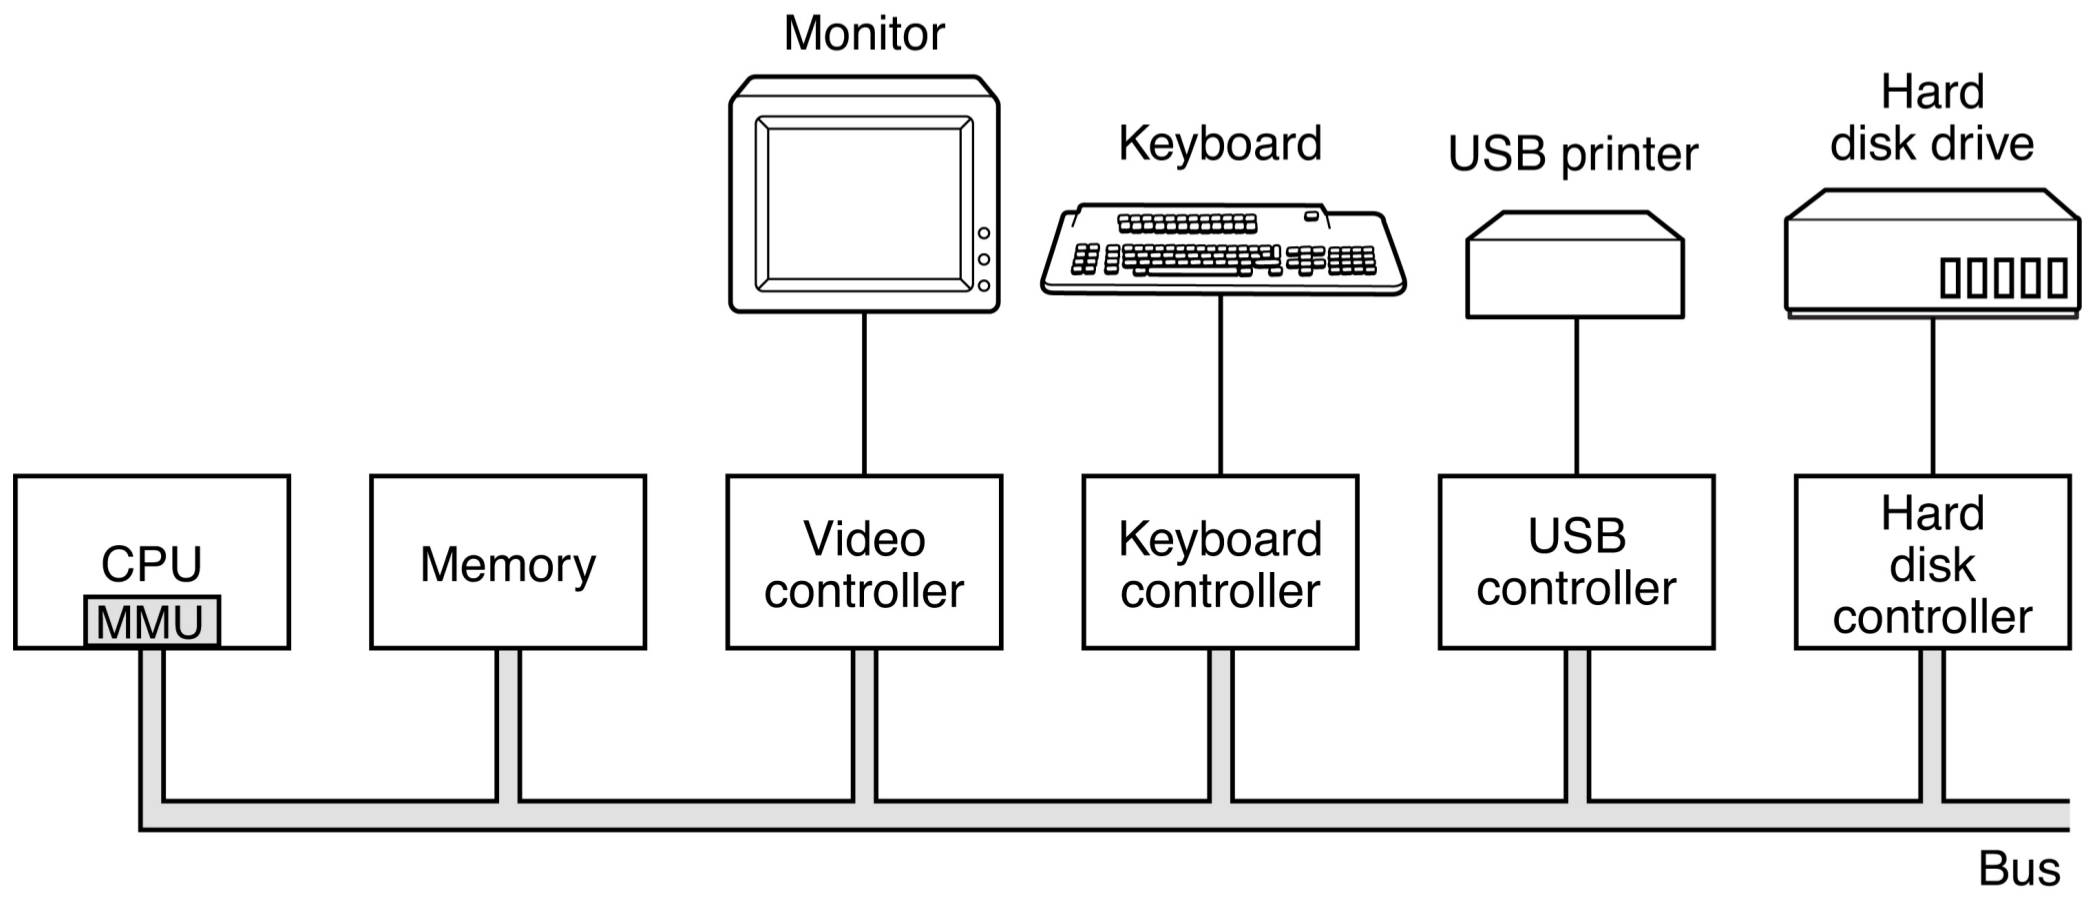
\includegraphics[width=0.33\textwidth]{BusSystem}\end{figure}
	\item today: multiple busses
	\begin{figure}[H]\centering\label{BusSystemToday}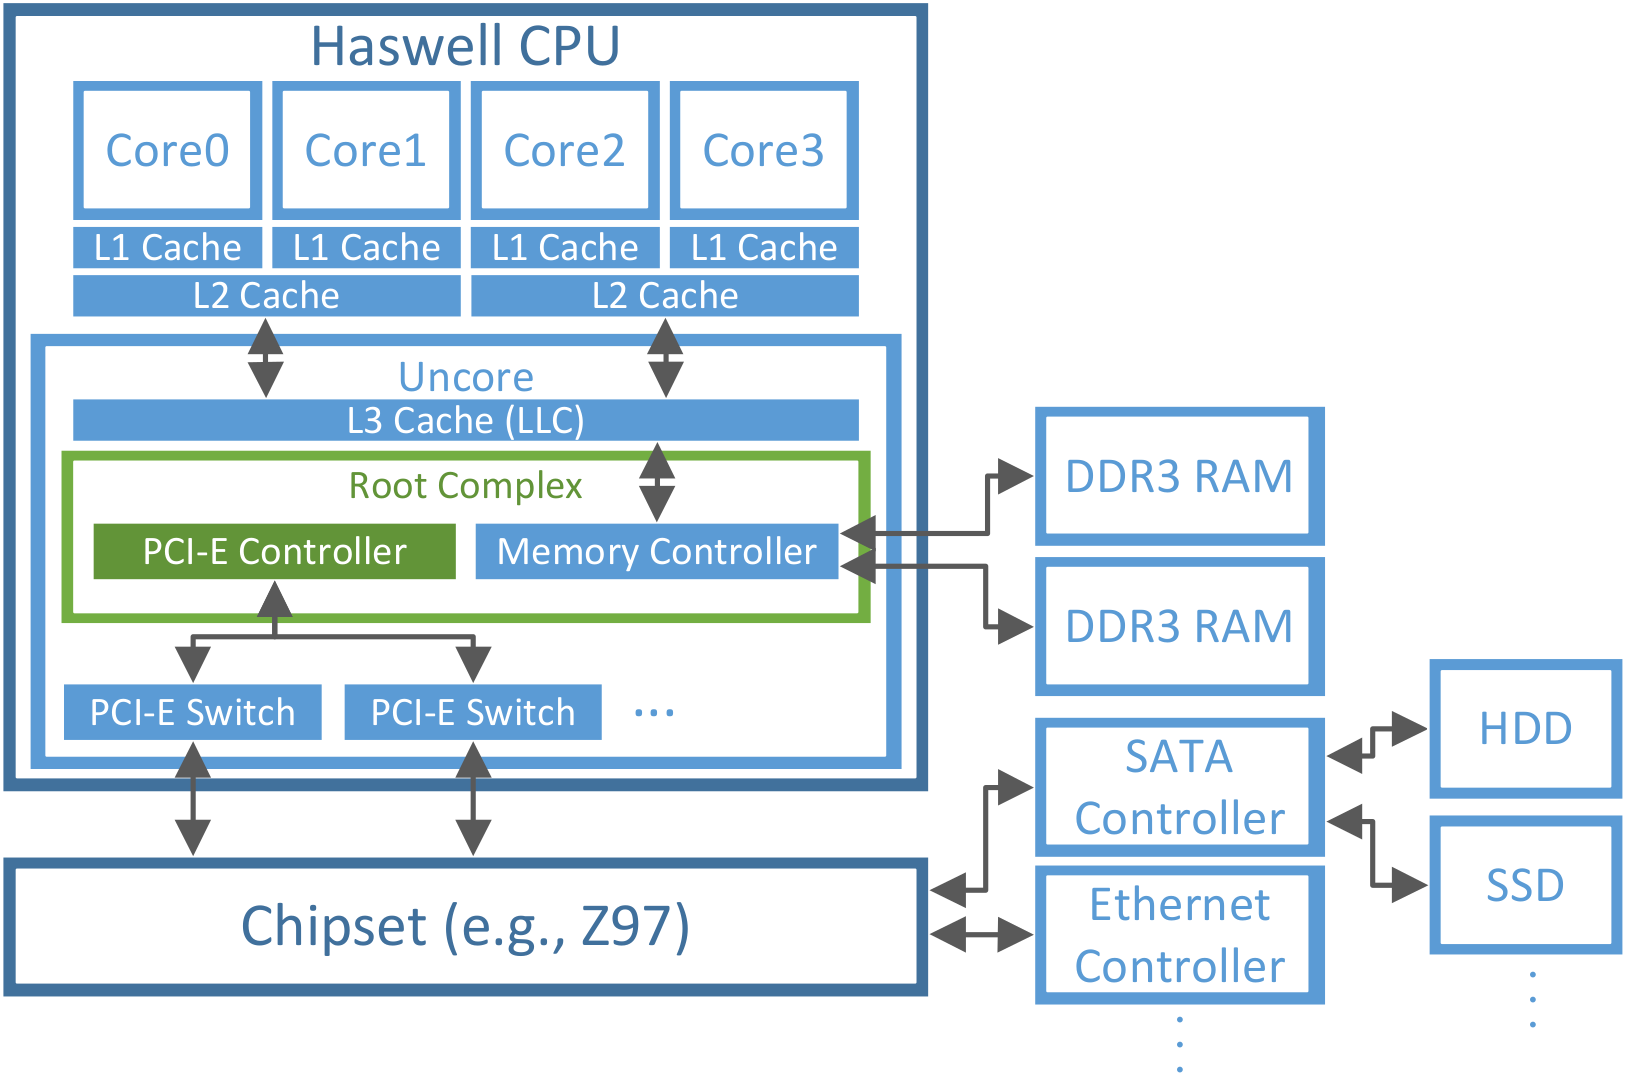
\includegraphics[width=0.33\textwidth]{BusSystemToday}\end{figure}
\end{items}

\paragraph{Central Processing Unit (CPU) --- Operation}
\begin{items}
	\item fetches instructions from memory, executes them (instruction format/-set depends on CPU)
	\item CPU internal registers store (meta-)data during execution (general purpose registers, floating point registers, instruction pointer (IP), stack pointer (SP), program status word (PSW),...)
	\item \textbf{execution modes}: \\*
		\textbf{user mode} (x86: \emph{Ring 3}/\emph{CPL 3}): \\*
			\phantom{x} only non-privileged instructions may be executed \\*
			\phantom{x} cannot manage hardware \( \to \) \textbf{protection} \\*
		\textbf{kernel mode} (x86: \emph{Ring 0}/\emph{CPL 0}): \\*
			\phantom{x} all instructions allowed \\*
			\phantom{x} can manage hw with \textbf{privileged instructions}
		\begin{figure}[H]\centering\label{OperationModes}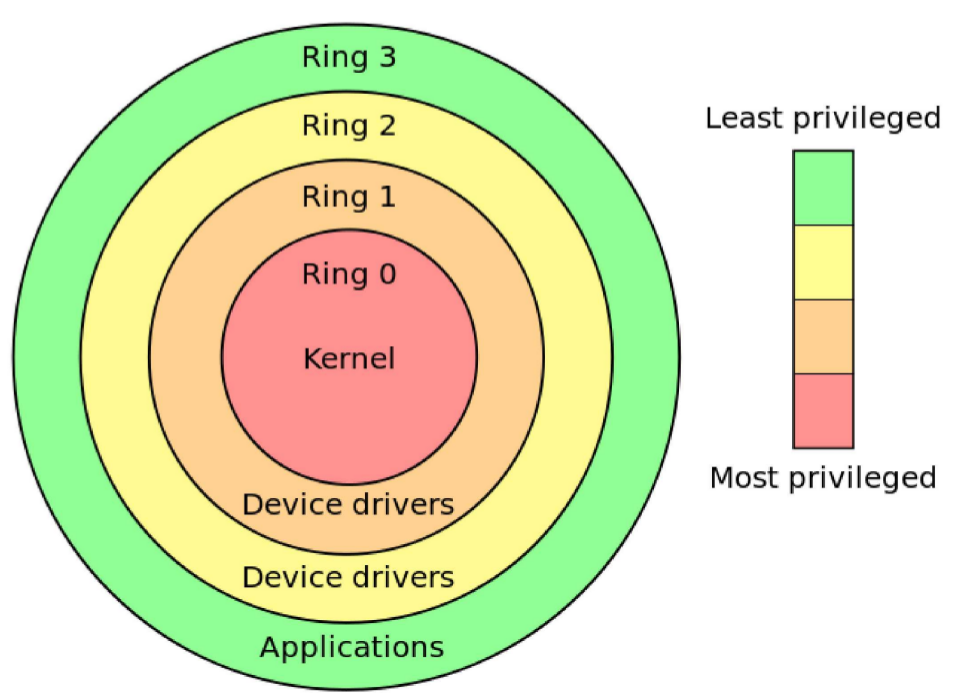
\includegraphics[width=0.2\textwidth]{OperationModes}\end{figure}
\end{items}

\paragraph{Random Access Memory (RAM)}
\begin{items}
	\item keeps currently executed instructions + data
	\item today: CPUs have built-in \emph{memory controller}
	\item root complex connected directly via \\*
		"`wire"' to caches \\*
		pins to RAM \\*
		pins to PCI-E switches
\end{items}

\paragraph{Caching}
\begin{items}
	\item RAM delivers instructions/data slower than CPU can execute
	\item memory references typicalle follow \emph{locality principle}: \\*
		\textbf{spatial locality}: future refs often near previous accesses \\*
			\phantom{x} (e.g. next byte in array) \\*
		\textbf{temporal locality}: future refs often at previously accessed ref \\*
			\phantom{x} (e.g. loop counter)
	\item \emph{caching} helps mitigating this memory wall: \\*
		copy used information temporarily from slower to faster storage \\*
		check faster storage first before going down \textbf{memory hierarchy} \\*
		if not, data is copied to cache and used from there
	\item \textbf{Access latency}: \\*
		register: \( \sim \)1 CPU cycle \\*
		L1 cache (per core): \( \sim \)4 CPU cycles \\*
		L2 cache (per core pair): \( \sim \)12 CPU cycles \\*
		L3 cache/LLC (per uncore): \( \sim \)28 CPU cycles (\( \sim \)25 GiB/s) \\*
		DDR3-12800U RAM: \( \sim \)28 CPU cycles + \( \sim \) 50ns (\( \sim \)12 GiB/s)
\end{items}

\paragraph{Caching --- Cache Organisation}
\begin{items}
	\item caches managed in hardware
	\item divided into \emph{cache lines} (usually 64 bytes each, unit at which data is exchanged between hierarchy levels)
	\item often separation of data/instructions in faster caches (e.g. L1, see \emph{harward architecture})
	\item \textbf{cache hit}: accessed data already in cache (e.g. L2 cache hit)
	\item \textbf{cache miss}: accessed data has to be fetched from lower level
	\item cache miss types: \\*
		\emph{compulsory miss}: first ref miss, data never been accessed \\*
		\emph{capacity miss}: cache not large enough for process working set \\*
		\emph{conflict miss}: cache has still space, but collisions due to \\* \phantom{x} placement strategy
\end{items}

\paragraph{Interplay of CPU and Devices}
\begin{items}
	\item I/O devices and CPU execute concurrently
	\item Each device controller \\*
		- is in charge of particular device \\*
		- has local buffer
	\item \textbf{Workflow}:
	\begin{enumeration}
		\item CPU issues commands, moves data to devices
		\item Device controller informs APIC (\emph{Advanced Programmable Interrupt Controller}) that operation is finished
		\item APIC signals CPU
		\item CPU receives device/interrupt number from APIC, executes handler
	\end{enumeration}
	\begin{figure}[H]\centering\label{CPUIOInterplay}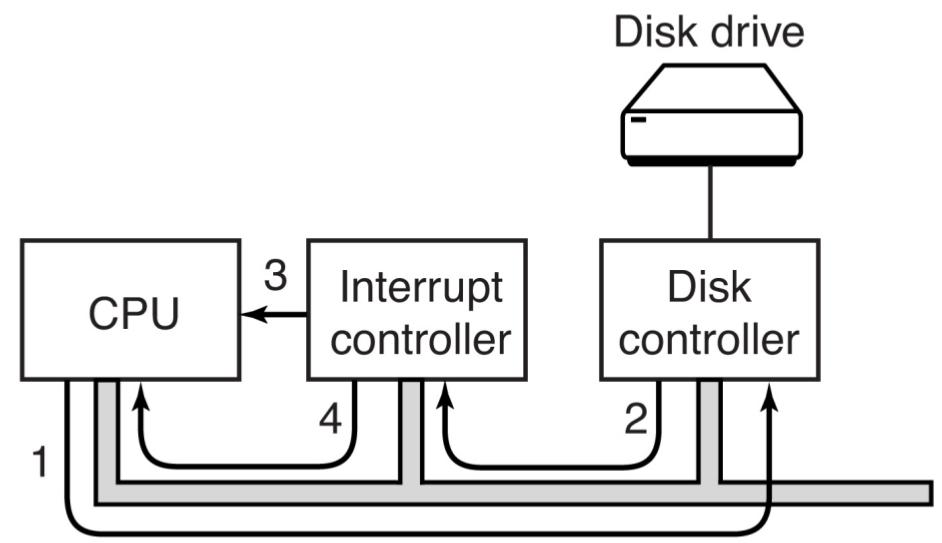
\includegraphics[width=0.2\textwidth]{CPUIOInterplay}\end{figure}
\end{items}

\newpage 

\paragraph{Device control}
\begin{items}
	\item Devices controlled through their \textbf{device controller}, accepts commands from OS via \textbf{device driver}
	\item devices controlled through device registers and device memory: \\*
		\emph{control} device by writing device registers \\*
		\emph{read} status of device by reading device registers \\*
		\emph{pass data} to device by reading/writing device memory
	\item 2 ways to access device registers/memory:
	\begin{enumeration}
		\item \textbf{port-mapped IO} (PMIO): \\*
			use special CPU instructions to access port-mapped \\* \phantom{x} registers/memory \\*
			e.g. x86 has different \code{in}/\code{out}-commands that transfer \\* \phantom{x} 1,2 or 4 bytes between CPU and device
		\item \textbf{memory-mapped IO} (MMIO): \\*
			use same address space for RAM and device memory \\*
			some addresses map to RAM, others to different devices \\*
			access device's memory region to access device registers/memory
	\end{enumeration}
	\item some devices use hybrid approaches using both
\end{items}

\paragraph{Device control --- Nvidia general purpose GPU}
\begin{items}
	\item memory-mapped ring-buffer and \code{put}/\code{get}-device
	\item mapping can be exposed to application \( \leadsto \) application can submit commands in user-mode
	\begin{figure}[H]\centering\label{NvidiaRing}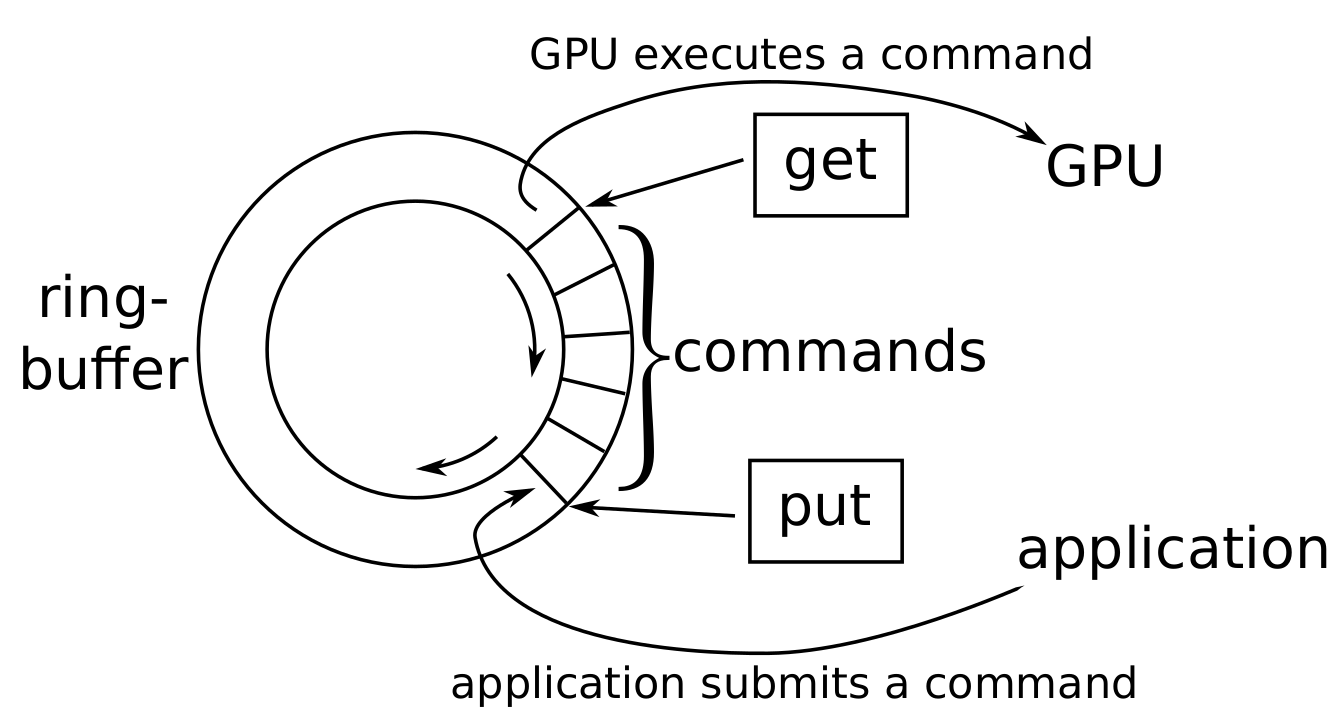
\includegraphics[width=0.33\textwidth]{NvidiaRing}\end{figure}
\end{items}

\begin{summary}
	\begin{items}
		\setlength\itemsep{0em}
		\item The OS is an abstraction layer between applications and hardware (multiplexes hardware, hides hardware details, provides protection between processes/users)
		\item The CPU provides a separation of User and Kernel mode (which are required for an OS to provide protection between applications)
		\item CPU can execute commands faster than memory can deliver instructions/data -- memory hierarchy mitigates this memory wall, needs to be carefully managed by OS to minimize slowdowns
		\item device drivers control hardware devices through PMIO/MMIO
		\item Devices can signal the CPU (and through the CPU notify the OS) through interrupts
	\end{items}
\end{summary}
